\documentclass[]{article}
\usepackage[]{apacite}
\usepackage{url} %this package should fix any errors with URLs in refs.
\usepackage{graphicx}
\usepackage{float}
\usepackage{mathtools}
\usepackage{amsmath}
\usepackage{amssymb}
\usepackage[export]{adjustbox}
%\let\citet\shortciteA
\usepackage[authoryear]{natbib}
\bibliographystyle{plainnat}
\usepackage[version=4]{mhchem}

%opening
\title{Modeling Gas Dynamics: Finite Volume Method Approach}
\author{Jacob Koile}

\begin{document}

\maketitle

\begin{abstract}
	Euler's equations of gas dynamics have been studied by all forms of science since their derivation in the time of Euler. In this paper, we focus on studying this famous set of coupled equations through a computational lens in order to take into account thermal ionization in the 2D streamer model by \citet{Liu:2004b}. The method we choose to use is based on Godunov's Method which uses the solution to the Riemann Problem. 

\end{abstract}

\section{The Euler Equations}

	We focus on the incompressible, inviscid, thermally non-conductive Euler Equations:

	\begin{equation}
	\frac{\partial\rho}{\partial t} + \nabla_{cyl} \cdot (\rho v) = 0
	\end{equation} 
	\begin{equation}
	\frac{\partial \rho v}{\partial t} + \nabla_{cyl} \cdot (\rho \textbf{V}^2 + p) = 0   
	\end{equation}
	\begin{equation}
	\frac{\partial \epsilon}{\partial t} + \nabla_{cyl} \cdot [(\epsilon + p)\textbf{V}] = Q_{eff}^T  
	\end{equation}	 
	\begin{equation}
	\epsilon = \frac{5}{2} N k_B T + \frac{1}{2}\rho \textbf{V}^2 
	\end{equation}
	\begin{equation}
	p = N k_B T
	\end{equation}

	Equation (1) accounts for mass transport (or is otherwise recognized as the mass continuity equation) where $\rho$ represents the mass density determined from all neutral species and $v$ is the bulk velocity. Equation (2) is the momentum density continuity equation accounting for Newton's Second Law by including the necessary contributions of pressure, $p$ as the surface force on the gas. Equation (3) is the translational energy continuity equation which accounts for the balance of its advection, its heat supply, $Q_{eff}^T$ (the effective rate of energy deposition) or Joule heating. Equation (4) is the equation. Equation (5) is the equation of state and closes the system.
	
	The equations above form a system of non-linear hyperbolic conservation laws that govern the dynamics of a compressible material, such as gases of liquids at high pressures, for which the effects of body forces, viscous forces, and heat flux are neglected. 
	
\section{Set-Up}
	We use the conservative form of the equations which follows the form:
	 
	\begin{equation}
		U_t + F(U)_x = 0
		\label{Gen_Hyp}
	\end{equation}
		\begin{align}
			U &= \begin{bmatrix}
				u_{1} \\
				u_{2} \\
				\vdots \\
				u_{m}
				\end{bmatrix} \mbox{,  } 
				F(U) = \begin{bmatrix}
				f_{1} \\
				f_{2} \\
				\vdots \\
				f_{m}
				\end{bmatrix} 
		\end{align}

	where U is a vector of conserved variables and F(U) is a vector of fluxes. To ``linearize'' the system, we introduce the flux Jacobian matrix,
	
	\begin{equation}
		A(U) = \frac{\partial F}{\partial U}.
		\label{HypSys}
	\end{equation}
	
	Now, the system is written in 'quasi-linear' form:
	
	\begin{equation}
		U_t + \frac{\partial F}{\partial U}\frac{\partial U}{\partial x} = U_t + A(U) U_x = 0.
		\label{QLHypSys}
	\end{equation}
	
	In order to solve this system we must first determine the eigensystem from the matrix
	
	\begin{equation}
		A K^{(i)} = \lambda_i K^{(i)}.
	\end{equation}
	
	This system is said to be hyperbolic if \textbf{A} has real eigenvalues $\lambda_i$ and a corresponding set of linearly independent right eigenvectors \textbf{K$^{(i)}$} for $i=1:m$, where \textit{m} is the number of equations. The system is strictly hyperbolic if all the eigenvalues are distinct.
	
	The eigensystem allows for the decoupling of the Euler equations, where the dependent variables U(x,t) are transformed into a new set of variables W(x,t). 
	
	First, we diagonalize \textit{A},
	
	\begin{equation}
		A = K \Lambda K^{-1}
	\end{equation}
	where $\Lambda$ is a matrix with the diagonal elements being the eigenvalues. To determine the new dependent variables \textbf{W}, we use the transformation
	\begin{equation}
		W = K^{-1} U  \mbox{ or }  U = KW.
	\end{equation}
	Now, substitute the equations (11) and (12) into equation (9) to get
	\begin{equation}
		W_t + \Lambda W_x = 0,
	\end{equation}
	which is called the characteristic form of the system and be written as 
	\begin{equation}
		\frac{\partial w_i}{\partial t} + \lambda_i \frac{\partial w_i}{\partial x} = 0 \mbox{,    } i = 1,...,m.
	\end{equation}

	Now this system is decoupled with $w_i$ being the single unknown, the characteristic speed is $lambda_i$, and there are m characteristics curves satisfying $m$ ODEs
	
	\begin{equation}
		\frac{dx}{dt} = \lambda_i, \mbox{for } i = 1,...,m.
	\end{equation}
	
	\subsection{Method of Characteristics}
	
		The characteristic curve discussed above is best described in the context of a scalar PDE such as
		\begin{equation}
			\begin{aligned}
			\mbox{PDEs} : u_x + au_t = 0 \mbox{, } -\infty 	< x < \infty \mbox{, } t > 0, \\
			\mbox{ICs}: u(x,0) = u_0(x).
			\end{aligned}
		\end{equation}
		A characteristic curve is defined as $ x = x(t) $ in the $ x-t $ plane along which the PDE becomes an ODE. So $ u(x(t),t) $ has a rate of change along $ x $ of 
		\begin{equation}
			\frac{du}{dt} = \frac{\partial u}{\partial t} + \frac{dx}{dt}\frac{\partial u}{\partial x}.
		\end{equation}
		If the characteristic curve $ x = x(t) $ satisfies the ODE
		\begin{equation}
			\frac{dx}{dt} = a
		\end{equation}
		then the PDE in equation (16) together with equation (17) gives
		\begin{equation}
			\frac{du}{dt} = \frac{\partial u}{\partial t} + a \frac{\partial u}{\partial x} = 0. 
		\end{equation}
		The time rate of change of $ u $ along the characteristic curve $ x = x(t) $ satisfying equation (18) is simply zero, implying $ u $ is constant along the characteristic curve. The speed $ a $ is called the characteristic speed and from equation (18) it is also the slope of the characteristic curve. For instance, if $ x(0) = x_0$, then the single characteristic curve that passes through the point ($ x_0, t=0 $) is
		\begin{equation}
			x = x_0 + at,
		\end{equation}
		which is shown in Figure \ref{CharacteristicCurve}.
		\begin{figure}[h] 	
			\centering
			%		\includegraphics[sc\left\{ ale=.30]{figures/GRLpaperFigures/Figure1_paper2_crossSectional.eps} %MSi
			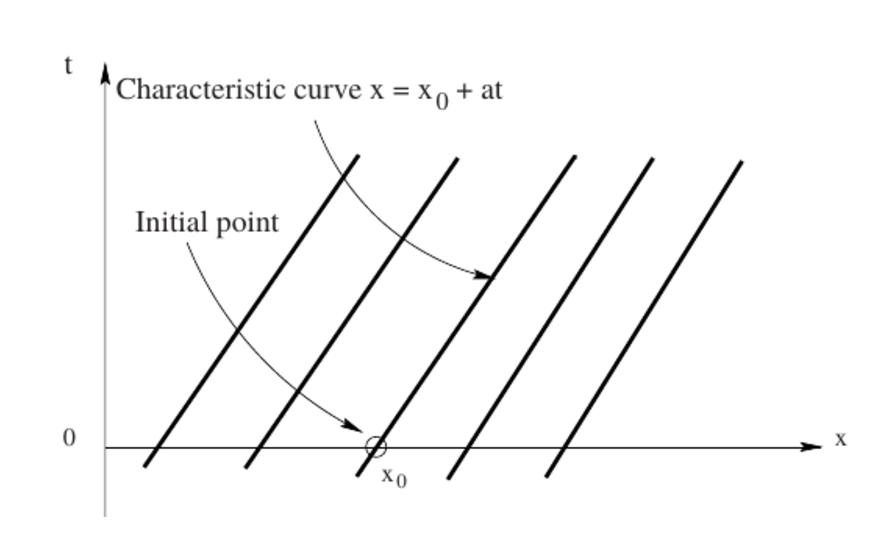
\includegraphics[scale=.50]{CharacteristicCurve}
			\caption{}
			\label{CharacteristicCurve}
		\end{figure} 	
		So, if $ u(x,0) = u_0(x) $ at $ t = 0 $, then along the characteristic curve, equation (20), the solution is
		\begin{equation}
			u(x,t) = u_0(x_0) = u_0(x-at).
			\label{general_sol}
		\end{equation}
		Put into words, \textit{given an initial profile $ u_0(x) $, the PDE will simply translate this profile with velocity $ a $}.
	
	\subsection{The General Initial Value Problem}
		Now, we go back to the general IVP, equation \ref{Gen_Hyp}, with initial data
		\begin{equation}
			U^{(0)} = (u_1^{(0)}, u_2^{(0)}, ..., u_m^{(0)})^T.
		\end{equation}
		We know from above that upon decoupling the equations, we get a solution like
		\begin{equation}
			w_i(x,t) = w_i^{(0)}(x - \lambda_i t), \mbox{for  } i = 1, 2, ..., m.
		\end{equation}
		The solution of the general IVP in terms of the original variables \textbf{\textit{U}} is obtained by the transform, as before, $ \textbf{U} = \textbf{KW} $. This in turn can be written as 
		\begin{equation}
			\textbf{U}(x,t) = \sum_{i = 1}^{m} w_i(x,t) \textbf{K}^{(i)}.
			\label{ind_waves}
		\end{equation}
		Explicitly, this shows that the function $ w_i(x,t) $ is the coefficient of $ \textbf{K}^{(i)} $ in an eigenvector expansion of the vector \textbf{U}. Thus, given a point $ (x,t) $ in the \textit{x-t} plane, the solution $ \textbf{U}(x,t) $ at this point depends only on the initial data at the \textit{m} points $ x_0^{(i)} = x - \lambda_i t $. The solution \ref{ind_waves} for \textbf{U} can be seen as the superposition of \textit{m} waves, each of which is advected independently without change in shape. The \textit{i}-th wave has shape $ w_i^{(0)}(x) \textbf{K}^{(i)} $ and propagates with speed $ \lambda_i $.
	
	\subsection{The Riemann Problem}
		The Riemann problem (RP) is a special initial value problem where a discontinuity exists between a grid wall as in Figure \ref{RiemannProblem}. The problem follows as:
		\begin{equation}
	    	\begin{aligned}
			\mbox{PDEs} : U_t + A U_x = 0\mbox{, } -\infty < x < \infty \mbox{, } t > 0 \\
			\mbox{ICs}: U(x,0) = U^{(0)}(x) = \left\{
			\begin{array}{ll}
			u_L & \quad x \leq 0, \\
			u_R & \quad x \geq 0.
			\end{array}
			\right.
		    \end{aligned}
		\end{equation}
	
		\begin{figure}[h] 	
			\centering
	%			\includegraphics[sc\left\{ ale=.30]{figures/GRLpaperFigures/Figure1_paper2_crossSectional.eps} %MSi
			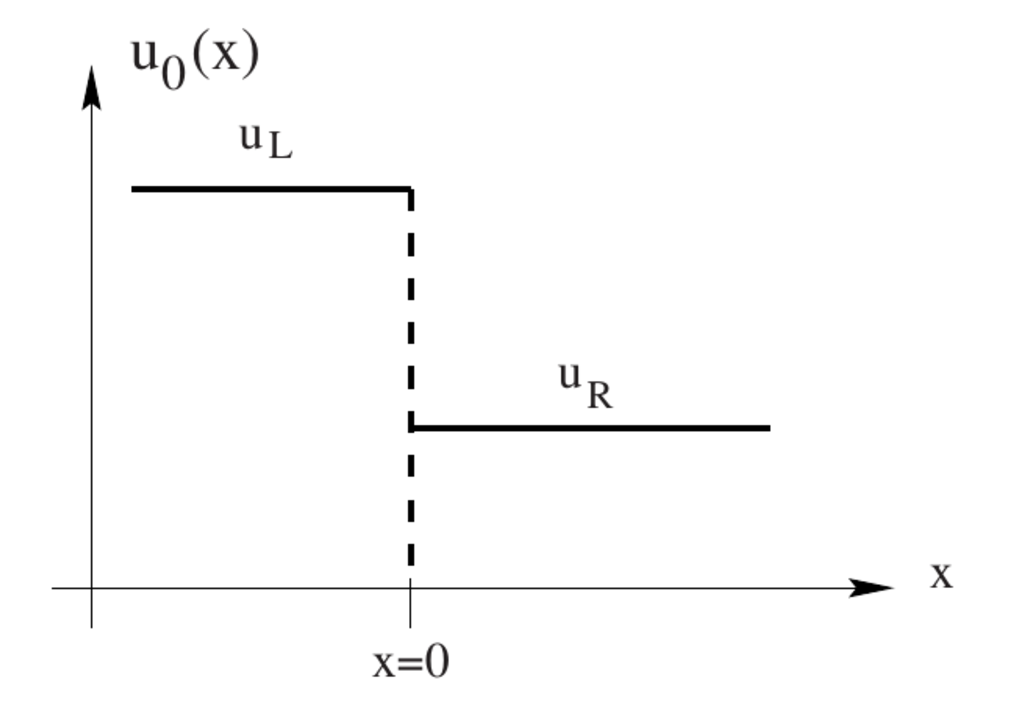
\includegraphics[scale=.30]{RiemannProblem}
			\caption{}
			\label{RiemannProblem}
		\end{figure} 
		The solution structure in the x-t plane is shown in Figure \ref{CharacteristicFanRP} where there are $ m $ waves propagating from the origin, one for each eigenvalue. These waves carry the jump discontinuity in $ U $ and propagate with speed $ \lambda_i $. It is simple to see that the solution the left of $ \lambda_1 $ is $ u_L $ and to the right of $ \lambda_m $ is $ u_R $. The problem is finding the solution in between these waves, a region known as the \textit{Star Region}. Since the eigenvectors are linearly independent, we expand the left and right data as linear combinations of the eigenvectors:
		\begin{equation}
			u_L = \sum_{i = 1}^{m} \alpha_i K^{(i)} \mbox{,   } u_R = \sum_{i = 1}^{m} \beta_i K^{(i)}.
			\label{right_left_exp}
		\end{equation}
		Where $ \alpha $ and $ \beta $ are constant coefficients. \textbf{Formally, the solution of the IVP is given by (\ref{ind_waves}) in terms of the initial data $ w_i^{(0)}(x) $ for the characteristic variables  and the right eigenvectors ($ K^{(i)} $}). \textit{Note that each of the expansions in (\ref{right_left_exp}) is a special case of (\ref{ind_waves})}.
	
		\begin{figure}[h] 	
			\centering
		%		\includegraphics[scale=.30]{figures/GRLpaperFigures/Figure1_paper2_crossSectional.eps} %MSi
			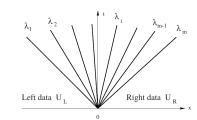
\includegraphics[scale=.30]{CharacteristicFanRP}
			\caption{}
			\label{CharacteristicFanRP}
		\end{figure} 	
		Equation (\ref{general_sol}) along with the initial data
		\begin{equation}
	    	\begin{aligned}
			w^{(0)}_i(x) &= \left\{
			\begin{array}{ll}
			\alpha_i & \quad \mbox{if } x \leq 0, \\
			\beta_i & \quad \mbox{if } x \geq 0
			\end{array}
			\right.
			\end{aligned}
		\end{equation}
		will have a solution given by
		\begin{equation}	    \begin{aligned}
			w_i(x,t) = w^{(0)}_i(x - \lambda_i t) &= \left\{
			\begin{array}{ll}
			\alpha_i & \quad \mbox{if } x - \lambda_i t \leq 0, \\
			\beta_i & \quad \mbox{if } x - \lambda_i t \geq 0.
			\end{array}
			\right.					
			\end{aligned}
		\end{equation}
		For a given point $ (x,t)$ there is an eigenvalue $ \lambda_I $ such that $ \lambda_I < \frac{x}{t} < \lambda_{I+1}$, which implies that $ x - \lambda_i t > 0 \mbox{ } \forall i \mbox{ }| \mbox{ } i \leq I$. So, we can now write the solution to the Riemann Problem in terms of the original variables as 
		\begin{equation}
			U(x,t) = \sum_{i = I+1}^{m} \alpha_i K^{(i)} + \sum_{i = 1}^{I} \beta_i K^{(i)},
		\end{equation}where the integer $ I = I(x,t) $ is the maximum value of the sub-index $ i $ for which $ x - \lambda_i t > 0 $.

	\subsection{Non-Linearities and Shock Waves}
		For non-linear hyperbolic conservation law systems, such as the case is with the Gas dynamics equations, the outcome has different properties when compared to the linear case. Using the basic initial value problem (IVP)
		\begin{equation}
			u_t + f(u)_x  \mbox{, } \mbox{  }u(x,0) = u_0(x),
			\label{IVP1}
		\end{equation} we explain these different properties in the following sections.
	
		\subsubsection{Construction of Solutions on Characteristics}
			Consider characteristics curves $ x = x(t) $ satisfying the IVP
			\begin{equation}
				\frac{dx}{dt} = \lambda(u) \mbox{, } x(0) = x_0,
				\label{2.88}
			\end{equation}
			where $ \lambda(u) = f'(u) $. By regarding both\textit{u} and \textit{x} as functions of \textit{t}, we find the total derivative  of \textit{u} along \textit{x(t)}, namely
			\begin{equation}
				\frac{du}{dt} = u_t + \lambda(u)u_x = 0.
			\end{equation}	
			In words, \textit{u} is constant along the characteristic curves satisfying (\ref{2.88}) and therefore the slope $ \lambda(u) $ is constant along the characteristic. Hence the characteristic curves are straight lines. The value of \textit{u} along each curve is the value of \textit{u} at the initial point $ x(0) = x_0 $ and so we write
			\begin{equation}
				u(x,t) = u_0(x).
				\label{analytSol1}
			\end{equation}
			Now the slope $ \lambda(u) $ of the characteristic may then be evaluated at $ x_0 $ so that the solution of the characteristics curves of the IVP (\ref{2.88}) are
			\begin{equation}
				x = x_0 + \lambda(u_0(x_0))t.
				\label{analytSol2}
			\end{equation}
			Equations (\ref{analytSol1}) and (\ref{analytSol2}) are the analytic solutions to the IVP. The point $ x_0 $ depends on the given point $ (x,t) $.
				
		\subsubsection{Wave Steepening and Shock Waves}
			The characteristic speed $ \lambda $ becomes $ \lambda(u) $, or a function of the solution which creates wave distortion. In Figure \ref{WaveDistortion}, we see a smooth initial profile with the initial data $ u_0 $ along with the initial points $ x_0 $. If we consider a convex flux function, $ \lambda^{'}(u) = f^{''}(u) > 0 $, then the characteristic speed  is an increasing function of $ u $. In the case of non-linear systems of conservation laws, the character of the flux function (convex, concave, or neither) is determined by the Equation of State.
	 
			\begin{figure}[h] 	
				\centering
		%		\includegraphics[scale=.30]{figures/GRLpaperFigures/Figure1_paper2_crossSectional.eps} %MSi
				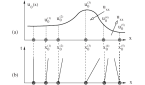
\includegraphics[scale=.50]{WaveDistortion}
				\caption{}
				\label{WaveDistortion}
			\end{figure}
			The higher values of $ u_0$ will therefore travel faster than the lower values. The region to the left of $ x_0^{(3)} $ is called the \textit{expansive region} and to the right is called the \textit{compressive region}. In the \textit{expansive region}, the characteristic speed $ \lambda_x > 0$ meaning as \textit{x} increases so to does the wave speed. Whereas in the \textit{compressive region} $ \lambda_x < 0 $. At a latter time, we would see that the expansive region will have a broader, flatter profile whereas the compressive region will tend to be steeper and narrower. When the characteristics in the compressive region intersect, the wave breaks or becomes a shock wave. A shock wave in air is a small transition layer of very rapid change of physical quantities such as pressure, density, and temperature. Breaking first occurs on the characteristic for which $ \lambda_x(x_0) $ is negative and $ |\lambda_x(x_0)| $ is a maximum.
	
			To take into account the shock wave, a formula is derived from the integral form of the conservation law system,
			\begin{equation}
				\frac{d}{dt}\int_{x_L}^{x_R}u(x,t)dx = f(u(x_L, t)) - f(u(x_R,t)),
			\end{equation}so that the shock wave can be modeled as a mathematical discontinuity (\textit{Shock Wave thickness can be an issue, see Landau and Lifshitz 1959 pp 337-341}). The formula is known as the \textit{Rankine-Hugoniot Condition},
			\begin{equation}
				\Delta f = S \Delta u,
				\label{RHC}
			\end{equation}
			where \textit{S} is the speed of the discontinuity. The equation algebraically relates the jumps between the the left and right fluxes, $ \Delta f $, the left and right conserved variables, $ \Delta u $, and the speed, $ S $, of the discontinuity.
	
		\subsubsection{The Entropy Condition}
	
			From the initial condition shown in  Figure \ref{ShockWave}(a), we see if the characteristic speed is a function of the data, then a shock wave will form immediately as seen from the characteristic curves shown in Figure \ref{ShockWave}(b). The discontinuous solution is a shock wave and is compressive in nature and must satisfy the following condition
			\begin{equation}
				\lambda(u_L) < S < \lambda(u_R),
			\end{equation}
			which is known as \textit{the entropy condition}.
			\begin{figure}[h] 	
				\centering
		%		\includegraphics[scale=.30]{figures/GRLpaperFigures/Figure1_paper2_crossSectional.eps} %MSi
				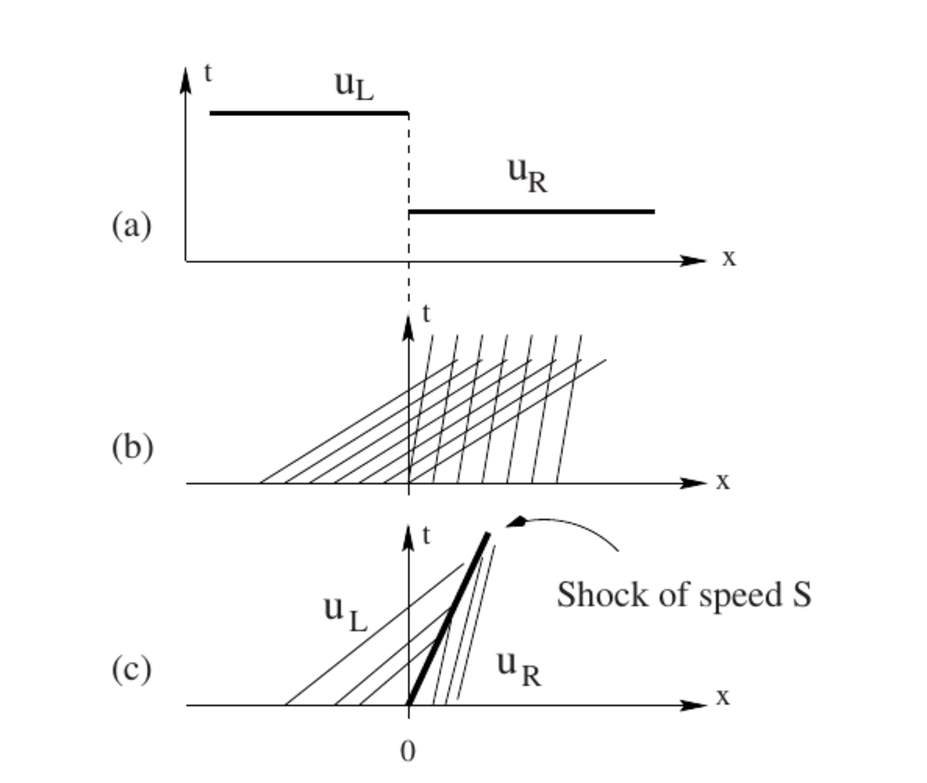
\includegraphics[scale=.50]{ShockWave}
				\caption{}
				\label{ShockWave}
			\end{figure}

		\subsubsection{Rarefaction Shock or Entropy-Violating Shock}
			If the data is flipped so it appears as \ref{RarefactionShock}(a), but the flux is still convex, Figure \ref{RarefactionShock}(b), a possible solution is the same as above, but will be violating the entropy condition, shown in Figure \ref{RarefactionShock}(c).
	
			\begin{figure}[h] 	
				\centering
		%		\includegraphics[scale=.30]{figures/GRLpaperFigures/Figure1_paper2_crossSectional.eps} %MSi
				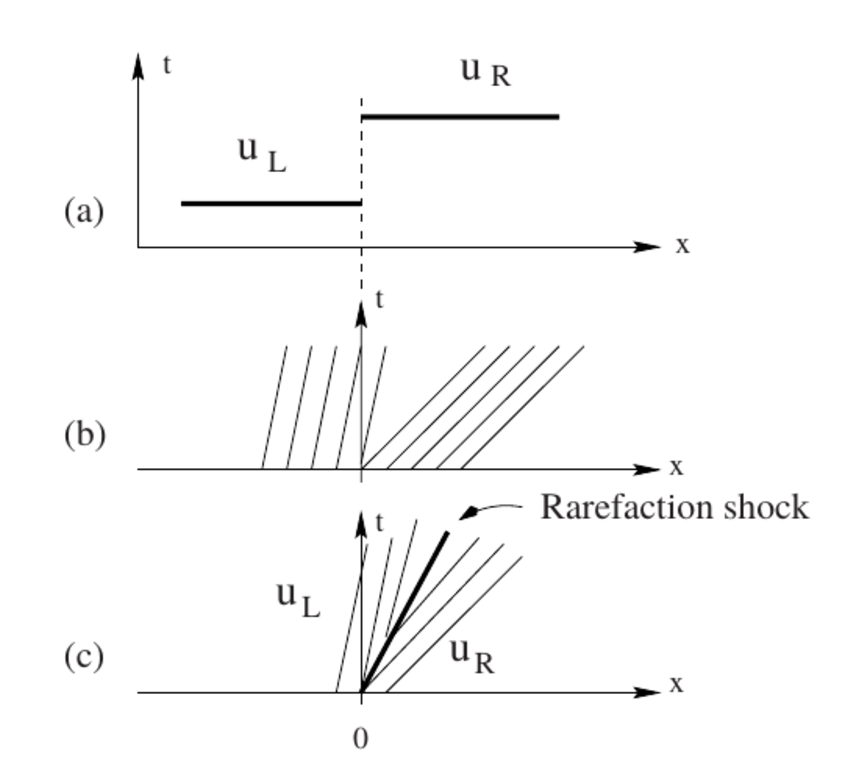
\includegraphics[scale=.55]{RarefactionShock}
				\caption{}
				\label{RarefactionShock}
			\end{figure}

		\subsubsection{Rarefaction Wave}
			By replacing the initial data with a linear variation between the discontinuity,
			\begin{equation}
				\begin{aligned}
					u_0(x) &= \left\{
						\begin{array}{ll}
							u_L & \quad \mbox{if } x \leq x_L, \\
							u_L + \frac{(u_R - u_L)}{(x_R - x_L} (x - x_L)  & \quad \mbox{if } x_L < x < x_R, \\
							u_R & \quad \mbox{if } x \geq x_R,
						\end{array}
					\right.
				\end{aligned}
			\end{equation}
			the solution to this problem is found by following characteristics which consists of two constant states, $ u_L \mbox{ and } u_R $, separated by a region of \textit{smooth transition}. This is called a \textit{rarefaction wave}. The right, \textit{head}, and left, \textit{tail}, edge of the wave in Figure \ref{RarefactionWave}(c) are given by the characteristics emanating from $ x_R \mbox{ and } x_L$, respectively. 

			\begin{figure}[h] 	
				\centering
		%		\includegraphics[scale=.30]{figures/GRLpaperFigures/Figure1_paper2_crossSectional.eps} %MSi
				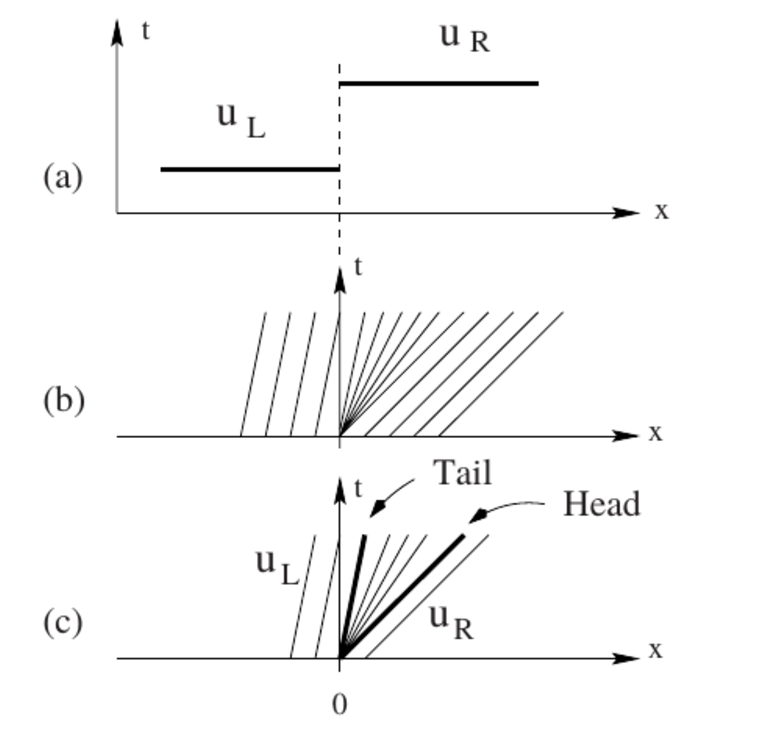
\includegraphics[scale=.55]{RarefactionWave}
				\caption{}
				\label{RarefactionWave}
			\end{figure}
			The spreading of waves a phenomenon not seen in linear hyperbolic systems with constant coefficients. The entire solution is
			\begin{equation}
				\begin{aligned}
				\left\{
					\begin{array}{ll}
						u(x,t) = u_L & \quad \mbox{if } \frac{x - x_L}{t} \leq \lambda_L, \\
						\lambda(u) = \frac{x - x_L}{t} & \mbox{if } \lambda_L < \frac{x - x_L}{t} < \lambda_R, \\
						u(x,t) = u_R & \quad \mbox{if } \frac{x - x_R}{t} \geq \lambda_R,
					\end{array}
				\right.
				\end{aligned}
			\end{equation}
	
			Now, there are at least two solutions to the IVP, equation \ref{IVP1}, which adds complexity due to the fact that one will be correct and the other spurious. How to distinguish between the two is by analyzing a physical discontinuity using the \textit{Rankine-Hugoniot Condition} and the \textit{entropy condition}.
	
		\subsubsection{Characteristic Fields}
			Consider the hyperbolic system of equation \ref{HypSys}. The characteristic speed $ \lambda_i(\textbf{U}) $ defines a characteristic field, the $ \lambda_i $-field or sometimes the $ K_i(\textbf{U}) $-field. By defining the gradient of the eigenvalue as
			\begin{equation}
				\nabla \lambda_i(\textbf{U}) = (\frac{\partial}{\partial u_1}\lambda_i, \frac{\partial}{\partial u_2}\lambda_i,..., \frac{\partial}{\partial u_m}\lambda_i)^T,
			\end{equation}
			we can determine the type of characteristic field as either \textit{Linearly Degenerate} or \textit{Genuinely Nonlinear}. Both defined as follows
			\begin{equation}
				\begin{aligned}
					\begin{array}{ll}
						\mbox{Linearly Degenerate} \\
						\nabla \lambda_i(\textbf{U}) \cdot \textbf{K}^{(i)}(\textbf{U}) = 0 \mbox{, } \forall\textbf{U} \in \Re^m
					\end{array}
				\end{aligned}			
			\end{equation}
			and
			\begin{equation} 
				\begin{aligned}
					\begin{array}{ll}
						\mbox{Genuinely Nonlinear} \\
						\nabla \lambda_i(\textbf{U}) \cdot \textbf{K}^{(i)}(\textbf{U}) \ne 0 \mbox{, } \forall\textbf{U} \in \Re^m,
					\end{array}
				\end{aligned}			
			\end{equation}
			where the $ \cdot $ represents the dot product in \textit{phase space}. The \textit{phase space} is space of vectors $ \textbf{U} $; for a $ 2x2 $ system it is the $ u_1-u_2 \mbox{ phase plane}$.
		
		\subsubsection{Rankine-Hugoniot Condtions}
			Using the same hyperbolic system as above with a discontinuous wave solution of speed $ S_i $ associated with the $ \lambda_i $-characteristic field, the Rankine-Hugoniot Condition (RHC), depicted in Figure \ref{RankineHugoniot}, is
			\begin{equation}
				\Delta F = S_i \Delta U.
			\end{equation}		
			\begin{figure}[h] 	
				\centering
			%		\includegraphics[scale=.30]{figures/GRLpaperFigures/Figure1_paper2_crossSectional.eps} %MSi
				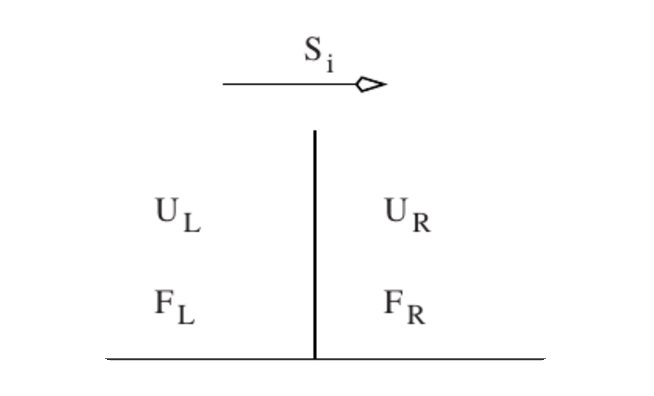
\includegraphics[scale=.55]{RankineHugoniot}
				\caption{}
				\label{RankineHugoniot}
			\end{figure}
			The \textit{RHC} can be used to determine the solution inside the \textit{Star Region}. For example, the linearized gas dynamics equations have an eigensystem
			\begin{equation}	
				U = [\rho, u] \mbox{ } \mbox{, }		
				\begin{aligned}
				\left[
					\begin{array}{ll}
						A = 0 & \rho_0\\
						\frac{a^2}{\rho_0} & 0 
					\end{array}
				\right]
				\end{aligned}
			\end{equation}
			and the eigenvalues
			\begin{equation}
				\lambda_1 = -a \mbox{, } \lambda_2 = a.
			\end{equation}
			Then by applying the \textit{RHC} across the $ \lambda_1 $-wave of speed $ S_1 = \lambda_1 $, we get
			\begin{equation}						
				\begin{aligned}
				\left[
					\begin{array}{ll}
						A = 0 & \rho_0\\
						\frac{a^2}{\rho_0} & 0 
					\end{array}
				\right]
				\end{aligned}
				\begin{aligned}
				\left[
					\begin{array}{ll}
						\rho^*-\rho_L \\
						u^* - u_L
					\end{array}
				\right]
				\end{aligned} =
				-a			
				\begin{aligned}
				\left[
					\begin{array}{ll}
						\rho^*-\rho_L \\
						u^* - u_L
					\end{array}
				\right].
				\end{aligned}
			\end{equation}
			By doing the same for the $ \lambda_2 $-wave of speed $ S_2 = \lambda_2 $, then expanding and solving both for $ u^* $, then with the two resulting equations we get the exact solution for the \textit{Star Region} unknowns.
		\subsubsection{Generlized Riemann Invariants}
			Consider the quasi-linear hyperbolic system of equation \ref{QLHypSys}, with
			\begin{equation}
				\textbf{W} = [w_1, w_2,..., w_m]^T.
			\end{equation}

			The \textit{Generalized Riemann Invariants} (GRI) are relations that hold true, for certain waves, across the wave structure and lead to the following $ m-1 $ ODEs
			\begin{equation}
				\frac{dw_1}{k_1^{(i)}} = \frac{dw_2}{k_2^{(i)}} = \cdots = \frac{dw_m}{k_m^{(i)}},
			\end{equation}
			where $ \textbf{K}^{i)} = [k_1^{(i)},...,k_m^{(i)}]$ is the corresponding eigenvector of the wave associated \textit{i}-characteristic field. The ODEs relate ratios of changes due to $ dw_s $ of quantities $ w_s $ to the respective eigenvector component corresponding to a $ \lambda_i $-wave family. With the same linearized gas dynamics equations as above, we use the GRI ODEs to find:
			\begin{equation}
				\begin{aligned}
					\begin{array}{ll}
						\mbox{Across the $ \lambda_1 $-wave} \\
						\frac{d\rho}{\rho_0} = \frac{du}{-a}
					\end{array}
				\end{aligned}			
			\end{equation}
			and
			\begin{equation} 
				\begin{aligned}
					\begin{array}{ll}
						\mbox{Across the $ \lambda_2 $-wave} \\
						\frac{d\rho}{\rho_0} = \frac{du}{a}.
					\end{array}
				\end{aligned}			
			\end{equation}
		
			After integrating these equations and applying them across the left wave, connecting the states $ W_L $ and $ W^* $, and the right wave, connecting the states $ W^* $ and $ W_R $, we get respectively
			\begin{equation}
				u^* + \frac{a}{\rho_0} \rho^* = u_L + \frac{a}{\rho_0}\rho_L
			\end{equation}
			\begin{equation}
				u^* - \frac{a}{\rho_0} \rho^* = u_R - \frac{a}{\rho_0}\rho_R.
			\end{equation}
			Solving both of these for the unknown variables, we get the same solution as above.
		
	\subsection{Elementary-Wave Solutions of the Riemann Problem}
		Now putting all of what we learned to use to solve a general $ m \mbox{x} m $ non-linear hyperbolic system with initial data
		\begin{equation}
			\begin{aligned}
				\textbf{U}_t + \textbf{F}(\textbf{U}) = 0 \mbox{, } \\
				U(x,0) = U^{(0)}(x) = \left\{
				\begin{array}{ll}
					\textbf{U}_L & \quad x < 0, \\
					\textbf{U}_R & \quad x > 0.
				\end{array}
			\right.
			\end{aligned}
			\label{RPEquation}
		\end{equation}
		The similarity solution $ \textbf{U}(x/t) $ of this system, consists of \textit{m+1} constant states separated by \textit{m} waves depicted in Figure \ref{ElementaryWaveSolutions}(A).
			
		\begin{figure}[h] 	
			\centering
			%		\includegraphics[scale=.30]{figures/GRLpaperFigures/Figure1_paper2_crossSectional.eps} %MSi
			\includegraphics[scale=.55]{ElementaryWaveSolutions}
			\caption{}
			\label{ElementaryWaveSolutions}
		\end{figure}
		For each eigenvalue, there is a wave family. If this a linear system with constant coefficients each wave is a discontinuity with speed $ S_i = \lambda_i $ and defines a linearly degenerate field.
		
		For non-linear systems, as described above, the waves may be discontinuities such as shock, contact, or rarefaction waves. The possible types of waves in the solution to the Riemann Problem depends critically on the closure conditions, that is to say the equation of state for the Gas Dynamics equations. Figure \ref{ElementaryWaveSolutions}(B) presents the three different wave types for a solution to the Riemann Problem that consists of a single non-trivial wave, where all other waves have zero strength.
		
		\subsubsection{Shock Waves}
			The two data states $ \textbf{U}_L $ and $ \textbf{U}_R $ are connected by a single jump discontinuity in a \textit{genuinely nonlinear field i} and the following conditions apply
			\begin{itemize}
				\item Rankine Hugoniot Conditions
				\begin{equation}
					\Delta \textbf{F}(\textbf{U}) = S_i \Delta \textbf{U}
				\end{equation}
				\item The Entropy Condition
				\begin{equation}
					\lambda_i(\textbf{U}_L) > S_i > \lambda_i(\textbf{U}_R).
				\end{equation}
			\end{itemize}
			This type of wave is shown in Figure \ref{ElementaryWaveSolutions}(B(a))		
		
		\subsubsection{Contact Waves}
			The two data states $ \textbf{U}_L $ and $ \textbf{U}_R $ are connected through a single jump discontinuity of speed $ S_i $  in a \textit{linearly degenerate field i} and the following conditions apply
			\begin{itemize}
				\item Rankine Hugoniot Conditions
				\begin{equation}
					\Delta \textbf{F}(\textbf{U}) = S_i \Delta \textbf{U}
				\end{equation}
				\item Constancy of the GRIs across the wave
				\begin{equation}
					\frac{dw_1}{k_1^{(i)}} = \frac{dw_2}{k_2^{(i)}} = \cdots = \frac{dw_m}{k_m^{(i)}},
				\end{equation}
				\item The parallel characteristic Condition
				\begin{equation}
					\lambda_i(\textbf{U}_L) = S_i = \lambda_i(\textbf{U}_R).
				\end{equation}
			\end{itemize}
			This type of wave is shown in Figure \ref{ElementaryWaveSolutions}(B(b)).
		
		\subsubsection{Rarefaction Waves}
			The two data states $ \textbf{U}_L $ and $ \textbf{U}_R $ are connected through a \textit{smooth transition region} in a \textit{genuinely nonlinear field i} and the following conditions are met
			\begin{itemize}
				\item Constancy of the GRIs across the wave
				\begin{equation}
					\frac{dw_1}{k_1^{(i)}} = \frac{dw_2}{k_2^{(i)}} = \cdots = \frac{dw_m}{k_m^{(i)}},
				\end{equation}
				\item Divergence of Characteristics
				\begin{equation}
					\lambda_i(\textbf{U}_L) <  \lambda_i(\textbf{U}_R).
				\end{equation}
			\end{itemize}
			This type of wave is shown in Figure \ref{ElementaryWaveSolutions}(B(a)
		
\section{Solving the Euler Equations}
	
	\subsection{Conservative versus Non-Conservative}
		First it is important to note two types of formulations of the Euler Equations. The most well known is the conservative form with
		
		\begin{equation}
			U_t + F(U)_x = 0
		\end{equation}
		\begin{align}
			U &= \begin{bmatrix}
			\rho \\
			\rho u \\
			E \\
			\end{bmatrix} \mbox{,  } 
			F(U) = \begin{bmatrix}
			\rho u \\
			\rho u^2 + p \\
			(E+p) u\
			\end{bmatrix},
			\label{EulerEquations}
		\end{align}
		where $ \rho $ is mass density, $ u $ is velocity, $ E $ is energy density, and $ p $ is pressure. The energy density equation is
		\begin{equation}
			E = \frac{1}{2}\rho(\textbf{V=$ < $u,0,0$ > $})^2 + \frac{p}{(\gamma -1)}.
		\end{equation}
		The conservation of mass, momentum, and energy are all well known physical laws. 
		
		A non-conservative form most commonly used is with the $ primitive-variables $. Which is found by expanding the derivatives in equation \ref{EulerEquations} which leads to, in quasi-linear form
		\begin{equation}
			W_t + A(W) W_x = 0
		\end{equation}
		\begin{align}
			W &= \begin{bmatrix}
			\rho \\
			u \\
			p \\
			\end{bmatrix}.
			\label{PrimitiveVariables}
		\end{align}	
		The conservative form is what we use mainly for the reason that \textbf{the solution to the non-conservative form that contains shock waves will give incorrect shock solutions.}
		
		
	\subsection{Characteristic Equations}
		
	\subsection{Elementary Wave Solutions of the Riemann Problem}
		
		The similarity solution of the Riemann Problem, equation \ref{RPEquation}, is depicted in Figure \ref{ElementaryWaveSolutions}(A), but in this case $ \lambda_i = \lambda_2$ and $ \lambda_m = \lambda_3$. The \textit{star-region} is located between $ \lambda_1 $ and $ \lambda_3 $. The two rays emanating from the wave solutions indicate that the character is still unknown. These three waves separate four constant states. In order to determine the wave-type, each type allowed in the solution, we first analyze the characteristic fields. We find that the $ \textbf{K}^{(2)} $-field is linearly degenerate, indicating this is a contact wave, and the $ \textbf{K}^{(1)} $ and $ \textbf{K}^{(3)} $ are genuinely non-linear, indicating that they can be a shock or rarefaction wave. One does not inherently know, beforehand, the types of waves present in the solution to the Riemann Problem. The only exception being the middle wave, which is always a contact discontinuity.
		
		\subsubsection{Contact Wave}
			A contact wave is a discontinuous wave across which both \textit{pressure} and \textit{velocity}, which is determined via the \textit{GRIs} for the $ \textbf{K}^{(2)} $-wave shown in equation \ref{GRIsK2}, are constant but density jumps discontinuously as do variables that depend on on density, such specific internal energy, temperature, speed of sound, entropy, etc.
			\begin{align}
				\textbf{K}^(2) &= \alpha_2 \begin{bmatrix}
				1 \\
				0 \\
				0 \\
				\end{bmatrix},
			\end{align}
			\begin{equation}
				\frac{d \rho}{1} = \frac{d(\rho u)}{u} = \frac{dE}{\frac{1}{2}u^2}
				\label{GRIsK2},
			\end{equation}
			where $ \alpha_i $ is the associated wave strengths.
			
		\subsubsection{Rarefaction Wave}		
			Inspecting the $ \textbf{K}^{(1)} $ and  $ \textbf{K}^{(3)} $ eigenvectors, shown in equation \ref{K1K3Prim}, for the primitive-variable formulation shows that $ \rho $, \textit{u}, and \textit{p} change across a rarefaction wave.
			\begin{align}
				\textbf{K}^(1) &= \alpha_1 \begin{bmatrix}
				1 \\
				-a/\rho \\
				a^2 \\
				\end{bmatrix},
			\end{align}
			\begin{align}
				\textbf{K}^(3) &= \alpha_3 \begin{bmatrix}
				1 \\
				a/\rho \\
				a^2 \\
				\end{bmatrix}.
			\end{align}
			In summary, a \textit{rarefaction wave} is a smooth wave associated with the 1- and 3-fields across which $ \rho $, \textit{u}, and \textit{p} change. The wave has a fan-type shape and is enclosed by two bounding characteristics. Across the wave the GRIs apply.
			
		\subsubsection{Shock Wave}
			Similar to the \textit{rarefaction wave}, across a \textit{shock wave} $ \rho $, \textit{u}, and \textit{p} change. Central to the analysis of a \textit{shock wave} is the application of the \textit{RHC}, where the shock speed can be determined. 
			
		\subsection{2D Euler Equations}
			Analyzing the 2D Euler Equations by making them quasi-linear and forming the eigensystem, we see that there are now four waves and four associated characteristic speeds. Similar to above, the $ \textbf{K}^{(1)} $ and $ \textbf{K}^{(4)} $ waves are genuinely non-linear and therefore associated with a \textit{shock} or \textit{rarefaction} wave. A difference lies now in the eigenvectors in the \textit{star region}, where $ \textbf{K}^{(2)} $ is a \textit{contact wave} so \textit{pressure} and \textit{velocity} are constant and \textit{density} jumps discontinuously across the wave and $ \textbf{K}^{(3)} $ is a \textit{shear wave} over which the \textit{tangential velocity} component jumps discontinuously across the wave.	
		
\section{Riemann Problem for Euler Equations}
	The key issues for designing an \textbf{Exact} \textit{Riemann Solver} are \begin{itemize}
		\item The variables selected
		\item The equations used
		\item The number of equations
		\item The technique for the iterative solutions
		\item The initial guess
		\item The way of handling unphysical iterates (i.e. negative pressures)
	\end{itemize}
		
\section{The Method of Godunov for Non-linear Systems}
		
\section{Approximate Riemann Solvers}
	The process of solving the RP is often quite expensive due to the necessary use of an iterative process to find solutions. The approximate, non-iterative solution provide the necessary items of information for numerical purposes at a fraction of the cost. The two approach types are \textit{approximation to the numerical flux} and \textit{approximation to a state}. The prior is what we use in Roe's Method.
		
	\subsection{Roe's Method}
	
		We begin by presenting Figure \ref{ARP IBVP} in which shows the general IBVP, followed by the solution written in the explicit conservative formula. The definition of the Godunov intercell numerical flux proceeds that and finally the solution to the IBVP is written in the general form.
		\begin{figure}[h] 	
			\centering
			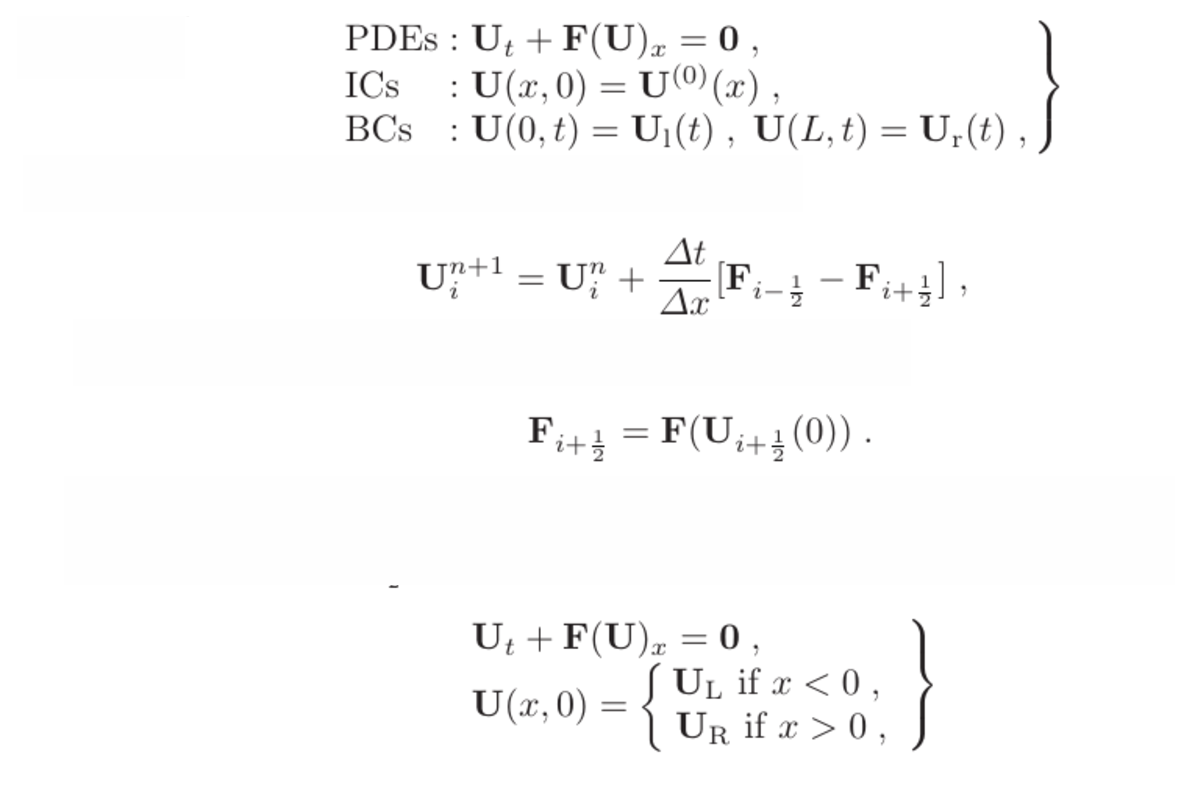
\includegraphics[scale=.50]{Approx_RP_GodFlux_IBVP}
			\caption{}
			\label{ARP IBVP}
		\end{figure}
		Where $ U_{i+1/2}(0) $ is the similarity solution $ U_{i+1/2}(x/t) $ of the Riemann problem evaluated at $ x/t $ = 0. The value $ x/t $ = 0 for the Godunov Flux corresponds to the $ t $-axis.
			
		\subsubsection{Failure of Roe's Method}		
		\subsubsection{Why impact to thermal ionization is not a highly energetic gas}
	\subsection{Transonic Waves}
	\subsection{Harten-Hyman Entropy Fix}
		Suppose there appears to be a transonic rarefaction wave
		
\section{end}

\bibliography{ref.bib}

\end{document}

